\documentclass{article}
\usepackage{graphicx} % Required for inserting images

% \usepackage{todonotes}
\usepackage[disable]{todonotes} % Uncomment to remove notes

%\usepackage[backend=biber,style=authoryear]{biblatex}
\bibliographystyle{apalike}
\bibliography{bibliography}



\title{Team Chocolate}
\author{Team Chocolate}
% \date{March 2025}

\usepackage{hyperref}

% % In case we HAVE TO use Arial
% \usepackage{fontspec}
% \setmainfont{Arial}



\begin{document}

\maketitle

\todo[inline]{Provide an overview of the proposed research, including background, rationale, objectives and goals, research design, team, and feasibility. Describe how the project includes the appropriate and explicit incorporation of community engagement, Indigenous science and technology studies, or EDI as appropriate. EDI related to the research team goes in the "EDI in Research Practice" section.
\\
Ensure that the project milestones and deliverables listed in the milestones and deliverable section are clearly described. Review the Application Guidelines to become familiar with evaluation criteria.}

% Airtable submission form: https://airtable.com/app8kmeGl0KXHFwoD/pagSpueY6HlZlI5ie/form

% Instructions: https://utoronto.sharepoint.com/:w:/s/vpresearch-external/CFREF/EeqXrJxtwc9GtNZXPGsj11wBXXqkYqo-kyyDDROReoFqbA?e=yhGoBT

\section{Introduction}

\section{Sub-project 1: Bibliometric Analysis}

Self-driving labs (SDLs) represent a new method of organizing research by combining automation, data science, and the scientific method to accelerate innovation in chemistry and materials science. Since the 1970s, articles have increasingly employed terms such as “autonomous laboratories,” “closed-loop experimentation,” and “materials acceleration platforms” (\cite{sterling2024}). However, the use of the term "self-driving laboratory" has exploded since 2020. As automation technologies become more widespread across the economy, there is a need to understand the trade-offs associated with their adoption and determine how organizations can optimally structure their research efforts. Analysis of bibliometric data on patterns of authorship and collaboration in SDL articles can offer novel insights into the organization of research.

A key issue emerging from the development of these technologies concerns the organization of collaborative research. As robots take on many of the research tasks traditionally performed by scientists and trainees, this raises questions about how researchers adapt, the optimal composition of expertise within a research team, and how automation may shift the notion of what constitutes an "optimal" research team. For instance, does automation substitute for human researchers, thereby reducing team size, or does it lead to larger teams by necessitating a broader array of specialized expertise? Additionally, it is important to determine which subfields are most significantly impacted by automation, and whether these effects vary based on researchers' backgrounds, such as academic versus industry experience.


The literature on team structure and productivity highlights several critical insights and complex dynamics relevant to these questions. Studies indicate that team size in science has grown due to an increasing "burden of knowledge" and specialization (\cite{jones2009burden}), yet smaller teams are more likely to achieve disruptive breakthroughs, while larger teams consolidate existing knowledge (\cite{wu2019large}). Moderately interdisciplinary research tends to have higher impact than either highly balanced or overly disparate interdisciplinary approaches \cite{yegros2015does}. Furthermore, teams comprising members who have not previously collaborated produce more original and multidisciplinary research (\cite{zeng2021fresh}), while flat, egalitarian teams outperform hierarchical ones in producing novel science (\cite{xu2022flat}).

The rise of AI and automation has the potential to disrupt these relationships, potentially allowing for different team compositions and combinations of expertise. For example, \cite{teodoridis2019creativity} emphasize that generalists excel creatively during periods of slow-paced knowledge change, while specialists thrive when rapid changes demand deeper, specialized expertise. \cite{Greska} finds that generalist teams outperform specialists in computer coding, though generative AI narrows this gap, potentially by reducing coordination costs. \cite{cavalli} studies scientists participating in the Critical Assessment of Protein Structure Prediction competition, and finds that the introduction of AlphaFold in 2018 led generalists to reduce the size of their labs, while specialist life scientists increased the size of their labs (mainly by hiring computer scientists).  Moreover, while automation and AI in scientific research enhance novelty and disruption, particularly in basic science (Chen, 2024), these gains appear complementary to domain expertise. \cite{tranchero2024finding} finds that pharmaceutical firms with substantial domain knowledge are less likely to invest in false positives generated by algorithmically-derived gene-disease relationships. Similarly, Toner (2024) identifies a risk of false positives in AI-enabled research, noting that more productive scientists are better equipped to harness this technology effectively. This highlights the crucial role of team members' prior backgrounds in filtering through the higher volume of potential findings in automated labs. 

SDL research projects differ in the degree of automation of both the software and data-driven decision-making aspect of the analysis, as well as in the automation of the experiments themselves.\cite{sterling2024} classifies these projects in a range from 1-5, with 5 assigned to fully automated projects along both dimensions (software and hardware). The optimal configuration of teams and researcher expertise and specialization in these projects presumably depends on the degree of automation.

Increasing automation also raises important questions about the role of different actors, i.e., students, postdoctoral researchers, and staff scientists, in this new paradigm. As robots perform tasks that would have historically been undertaken by students or postdocs, what are the implications for the training of the next generation of scientists? Does the adoption of automation reduce the demand for postdocs? Or does it increase demand for postdocs with greater computational expertise? What is the role of staff scientists, and how will they be motivated and rewarded as labs become more automated? Furthermore, there may also be implications for the gender composition of research teams as automation domain knowledge from male-dominated fields like computer science and engineering becomes more valuable as the technology is adopted in traditionally more gender-balanced fields such as the life sciences. 


%\begin{figure}
 %   \centering
  %  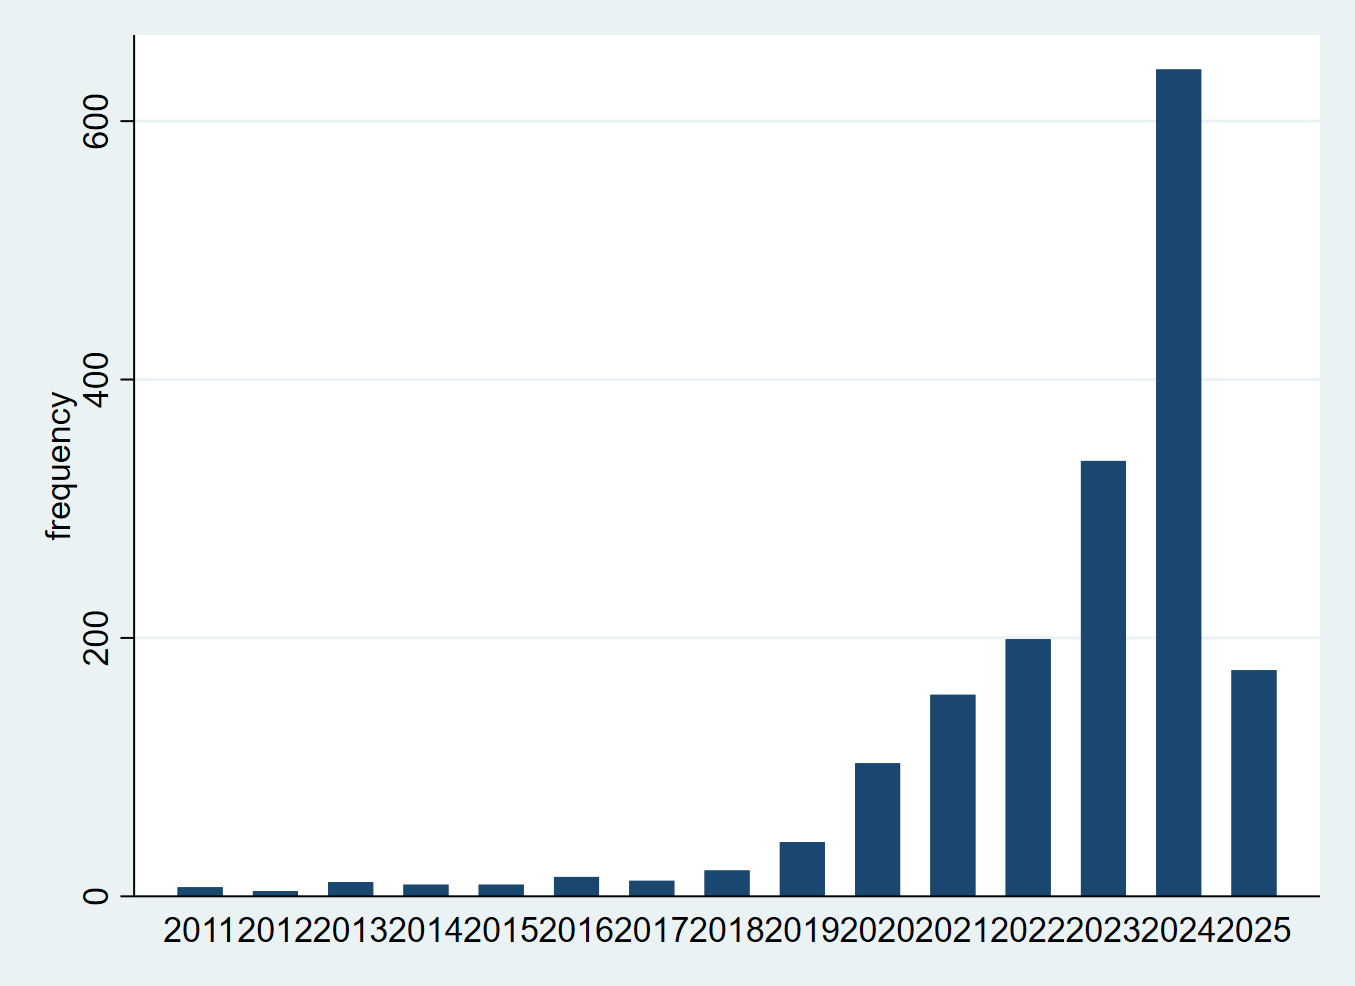
\includegraphics[width=0.75\linewidth]{count_by_year.png}
   % \caption{Number of SDL articles indexed by Dimensions.ai, by publication year. 
    %Includes articles that reference the terms "self-driving laboratory", "autonomous laboratories,” “closed-loop experimentation,” or “materials acceleration platforms.”}
     %  \label{fig:counts}
%\end{figure}

%The emergence of these technologies raises questions about how researchers respond, the optimal mix of expertise on a research team, and the tradeoffs that might shift what is ``optimal" in certain contexts. For example, does automation substitute for researchers, reducing the size of research teams? Or, does it increase team size because this research requires a larger number of specialists in different research fields? In which sub-fields does automation have the biggest impact? Do the effects vary by the background of the researchers (e.g., academic versus industry experience)? What are the impacts on training the next generation of researchers?

%Prior research on the introduction of new automation and artificial intelligence tools in scientific research has suggested that the use of AI-related terms in a corpus of scientific articles is associated with greater novelty and disruption, with the strongest effects in basic science \cite{chen2024}. \cite{tranchero2024finding} finds that pharmaceutical firms possessing greater domain knowledge are less likely to invest in false positives generated by algorithmically-derived gene-disease relationships (GWAS). This points to an important role for prior backgrounds in sifting through the higher volume of potential findings in automated labs. \cite{toner2024artificial} also finds a risk of false positives in AI-enabled research, with more-productive scientists better able to leverage the technology.

%The literature on team size and productivity more generally has found that team size in science has risen as the ``burden of knowledge" has become larger, and researchers have become more specialized \cite{jones2009burden}. Other work has found that smaller research teams are more likely to produce disruptive breakthroughs, while larger teams tend to work on consolidating the results of these breakthroughs  \cite{wu2019large}. [ADD MORE RELEVANT STUFF HERE] 

%The rise of AI and automation has the potential to disrupt these relationships, potentially allowing for different team compositions and combinations of expertise. For example, \cite{teodoridis2019creativity} emphasize that generalists excel creatively during periods of slow-paced knowledge change, while specialists thrive when rapid changes demand deeper, specialized expertise. \cite{Greska} shows that teams of generalists outperform specialists in computer coding; however, the introduction of generative AI reduced this performance differential (possibly by reducing coordination costs). \cite{cavalli} studies scientists participating in the Critical Assessment of Protein Structure Prediction competition, and finds that the introduction of AlphaFold in 2018 led generalists to reduce the size of their labs, while specialist life scientists increased the size of their labs (mainly by hiring computer scientists).  

%SDL research projects differ in the degree of automation of both the software and data-driven decision making aspect of the analysis, as well as in the automation of the experiments themselves.\cite{sterling2024} classifies these projects in a range from 1-5, with 5 assigned to fully automated projects along both dimensions (software and hardware). The optimal configuration of teams and researcher expertise and specialization in these projects presumably depends on the degree of automation.

%Increasing automation also raises important questions about the training of scientists. As robots perform tasks that would have historically been undertaken by students or postdocs, what are the implications for the training of the next generation of scientists? Does the adoption of automation reduce the demand for postdocs? Or does it increase demand for postdocs with greater computational expertise? What is the role of staff scientists, and how will they be motivated and rewarded as labs become more automated?

%Age-biased technical change is a rising concern, as well. The vintage of certain types of human capital can affect what types of workers are complementary to new technologies \cite{chari1991vintage, barth2023twisting}). While individual-level data on age are typically problematic to acquire and manage, understanding how experience--which is often visible in professional profiles---shapes scientists' ability to leverage automation may pick up the same mechanisms. We anticipate that this variation will have profound implications for hiring, training, and promotion of researchers as SDL technology diffuses.  There may also be implications for the gender composition of research teams as automation domain knowledge from male-dominated fields like computer science and engineering becomes more valuable as the technology is adopted in traditionally more gender-balanced fields such as the life sciences. 

%\begin{figure}
 %   \centering
  %  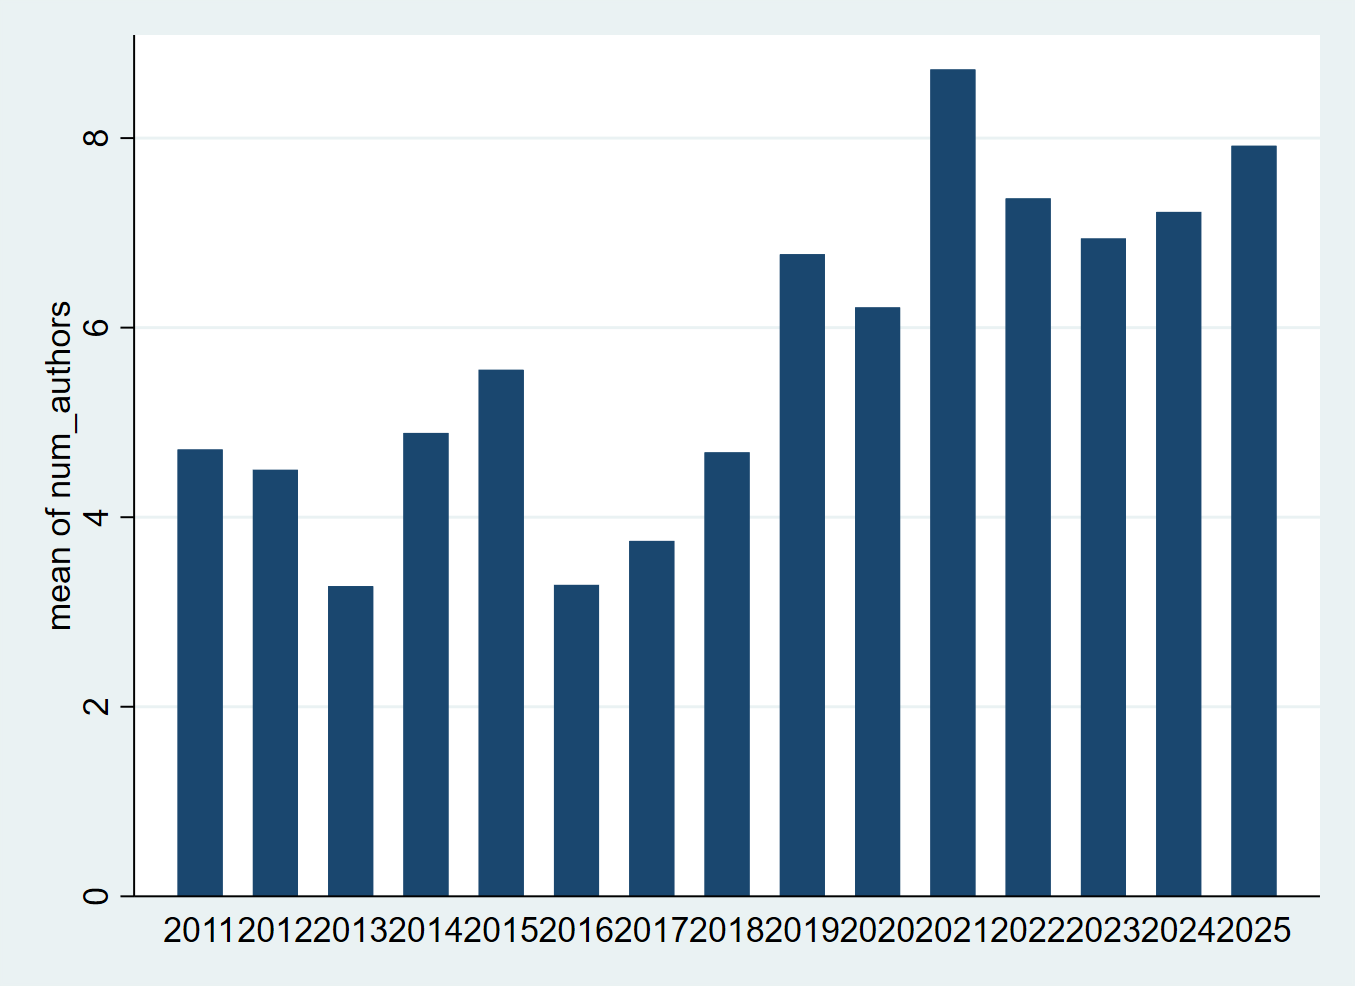
\includegraphics[width=0.75\linewidth]{num_authors.png}
   % \caption{Average number of authors on SDL papers, by year}
    %\label{fig:team size}
%\end{figure}

%\begin{figure}
 %   \centering
  %  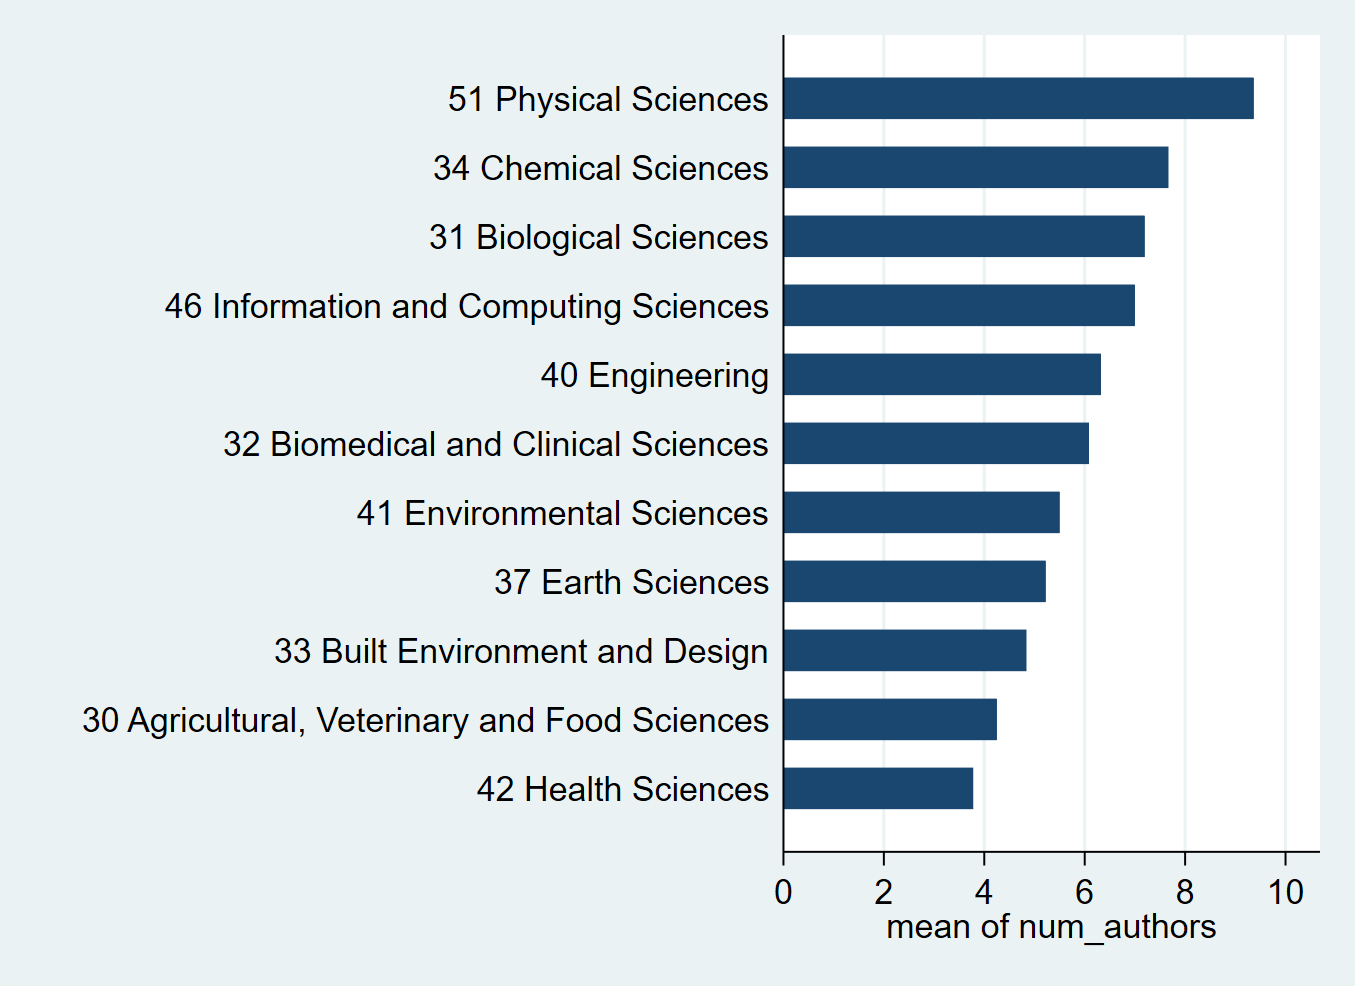
\includegraphics[width=0.75\linewidth]{num_authors_by_1stfield.png}
   % \caption{Average number of authors by first-listed research field in sample of SDL articles }
    %\label{fig:authors by field}
%\end{figure}

We propose to use bibliometric data on SDL projects to answer several descriptive questions about the organization of research. Preliminary evidence on the average number of authors on an SDL-related paper\footnote{Identified using the keywords listed above.} suggests that the average team size has risen from 3.4 prior to 2015 to 7.1 in 2015 or later.  The number of authors per paper varies across research fields, with the largest teams in the physical and chemical sciences.
%The most common author country of origin in the sample is the United States, with 29.7\% of articles, followed by China with 9.2\% and Canada with 8.3\%.  


\begin{enumerate}
    \item Do smaller SDL teams produce more novel or important research than larger teams? 
    \item Do more specialized SDL teams produce more novel or important research?
    \item How does the mix of disciplinary expertise affect outcomes in SDL teams? Does this vary by sub-field?
    \item What can we say about the distribution of experience in SDL teams? Is automation better leveraged by more or less-experienced researchers?
\end{enumerate}
Our goal is to provide insight into causal relationships between team composition and research output. Estimating causal effects from observational data typically requires a quasi-experimental a identification strategy, because research team composition may be determined by unobserved factors correlated with the outcomes of the research. For example, principal investigators on higher-potential research projects might recruit larger and more scientifically diverse teams for projects with greater unobserved scientific potential.

In order to control for this unobserved heterogeneity, we propose to exploit the COVID-19 shock to the research environment, which affected physical access to laboratories differently in different locations, in ways unrelated to the underlying  scientific opportunity in the location. As shown by \cite{broady2023automation}, the pandemic increased adoption of automation in the broader economy. We physical access limitations reduced the relative cost of automating tasks in laboratories and led labs to adjust their research projects to prioritize tasks that could be performed remotely, while teams in locations without COVID-related access restrictions had weaker incentives to automate tasks.  
\begin{enumerate}
    \item How did the pandemic restrictions affect the   degree of automation and the composition of SDL research teams?
    \item How did the variation in team composition caused by pandemic restrictions affect the nature of research outputs?
\end{enumerate}

The results of this analysis will inform the design of sub-project 2 (the experimental research).
\subsection{Data and Methodology for Sub-project 1}
We propose to collect bibliometric data from OpenAlex to comprehensively capture SDL-related publications, employing a dictionary-based method to identify these papers by developing a vocabulary of SDL-specific terms. Team size will be determined by the number of authors per paper. Each author will be linked to their publication history in OpenAlex to assess their specialization, allowing us to evaluate team composition. Specialization will be measured in two ways: first, by aggregating OpenAlex-annotated fields per author; second, by calculating the cosine similarity between author pairs and examining team variance, capturing diversity both within and across fields. SDL outputs will be measured by academic citations and broader scientific or commercial impacts through patent linkages (\cite{marx2020reliance}). Additionally, CV data from SDL authors will help analyze their career mobility and trajectories, assessing labor demand characteristics (e.g., academia versus industry) and the influence of SDL experience on their professional paths, and conducting gender disparity analyses inferred from profile images or names. This bibliometric approach will enable a global analysis of SDL research outputs across institutions and countries.

%We also propose to use  UMETRICS from the Institute for Research on Innovation and Science (IRIS), which contains richly detailed administrative data  on scientific research activities, funding, staffing, and expenditures at 45 large US research universities. This data, while limited to a subset of institutions, allows for a much more fine-grained and comprehensive analysis of the complete research process at an institution. For example, it allows us to separately identify salaries paid to faculty, postdocs,  students, and staff, as well as expenditures on scientific supplies and equipment and information technology. By combining this data with publication-based measures, we can examine how the allocation of expenditures toward physical vs. human capital affects research productivity in SDLs.

\subsection{Budget/Resources required for Sub-project 1}
\begin{enumerate}
    \item Research assistant to help with data collection and dataset construction
    \begin{enumerate}
        \item We will use data from OpenAlex, which is publicly available, but requires some programming to turn into a dataset for analysis. We anticipate that this will require one month of full-time summer RA work.
    \item To examine the effects on traditional laboratory members, we will collect CV data from SDL authors through databases such as \textcolor{red}{Revelio (at an estimated cost of \$20,000) or Core Signal (pricing available at https://coresignal.com/pricing/)}. After obtaining access, specific data requests must be submitted to these providers, and subsequent data processing will require dedicated support. We anticipate that processing this data will require three months of full-time summer research assistance.
    \end{enumerate}
\end{enumerate}
2. OTHER? Travel to conferences?



\section{Sub-project 2: Experiment}


% How would you quantify degree of automation/autonomy?

% E.g., classifying levels of autonomy (AI vs. automation grid)
% Turing test benchmark for AI quality

% Gerbrand Ceder - 30 million, 30 people, 3 years. Great robotics and automation, less impressive outcome.

% Pastry chef on teams. Dietetics.

% budget of 10 cocoa cores
% 1 month to build the system and collect data
% Notify in advance that after one month, they will be given a new chocolate formulation to optimize


Vary the team composition and look at the amount of automation and sophistication of AI in the experiment

At this point, there are a number of potentially interesting and important outcomes of interest:
\begin{itemize}
    \item  degree of automation
    \item  sophistication of AI
    \item  properties of chocolate
    \item  creating a system that maximizes the value of the experiment and reduces the burden
    \item  building a robust system for experimenting
    \item number of hours spent in project?
    \item  building a system that is flexible (can make more than one type of chocolate)...this is where the value of AI comes in, so you don't have to reinvent the wheel for every new experiment
    \item experience of people on the team
    \item 
\end{itemize}
That said, we will ultimately have to narrow this down based on the bibliometric study and our power calculations (i.e., how many participants we can expect in the hack-a-thon and expected effect sizes).

How will we vary team composition?
\begin{itemize}
\item {educational background}
\item{specialist vs. generalist (people with both CS and domain experience)}
\item{industry experience}
\item{team size}
\item{is there someone on the team who has taken Sterling's course?}
\item{pastry chef??}
\end{itemize}

\section{Impact and alignment}
The diffusion of SDLs is happening without people really knowing how to organize teams. Anecdote about CA lab. We will remove frictions of forming teams by providing insight into what works.

SOME THOUGHTS (KM):

This project directly advances the Acceleration Consortium's vision by addressing a critical challenge in self-driving labs: how to structure the human teams that design and operate them. By combining bibliometric analysis of successful automated discovery teams with experimental testing of team compositions, we will develop evidence-based insights that enhance how materials scientists collaborate with AI systems.

Our work aligns with multiple AC goals: First, by identifying preferred team structures for self-driving labs, we directly support the Consortium's mission to combine materials science with AI and robotics for accelerated discovery. Second, our project contributes to upskilling researchers by identifying the interdisciplinary competencies and collaborations needed in successful teams. Third, our interest in tradeoffs between specialist domain experts and generalist "bilinguals" in these teams addresses the organizational economics of this form of human-AI collaboration. Finally, examining the training and diversity implications speaks to key sustainability and ethical concerns, as well.

The project's innovative experimental approach using chocolate 3D printing creates a controlled environment to test team dynamics while also building actual skills in automation and materials design among participants. By focusing on the human element of self-driving labs, our project complements the Consortium's technical research, ensuring investments in advanced equipment and AI are maximized through optimal team configurations.


\subsection{Part of the proposal}
\begin{itemize}
    \item Proposal is 3 pages (11 pt font) (Marlène and Megan on the part of bibliometric part)
    \item Team Justification and EDI statement (2000 characters)
    \item Impact and Alignment Statement (1000 characters)
    \item Milestones and Deliverables (1500 characters)
    \item Total Budget (Sterling and Kristina)
    \item Budget justification (1500 characters)
\end{itemize}
Link to submission details: \href{https://airtable.com/app8kmeGl0KXHFwoD/pagSpueY6HlZlI5ie/form}{https://airtable.com/app8kmeGl0KXHFwoD/pagSpueY6HlZlI5ie/form}

\bibliography{bibliography}

% "List key milestones and deliverables in a list with a timeline (maximum 1500 characters). Please note that milestones should be described in the proposal and situated in the research context. This section is just a list of the milestones and deliverables."

\subsection{Timeline and Outcomes}
\begin{description}
  \item[05-06/25]: Recruit and train RAs; source data; develop LLM extraction tools for bibliometric study; begin hack-a-thon experiment design
  \item[Milestone]: Computational infrastructure for bibliometric analysis, refined analysis plan

  \item[07-08/25]: Conduct bibliometric data extraction; develop chocolate 3D printing challenge; prepare experimental protocols; source materials and pilot experiment (August)
  \begin{itemize}
    \item[Milestone]: Descriptive bibliometric statistics; pilot hack-a-thon with 2-3 teams
  \end{itemize}

  \item[09-11/25]: Complete bibliometric analysis; refine hack-a-thon protocols based on this and pilot results
  \begin{itemize}
    \item[Milestone]: Finalized team composition hypotheses
    \item[Deliverable]: Pre-registration of experimental protocols and analysis plan; submission for ethics approval; working paper based on bibliometric findings.
  \end{itemize}

  \item[12/25 - 05/26]: Recruit participants; prepare materials; run experiment
  \begin{itemize}
    \item[Milestone]: Hack-a-thon execution and data collection
  \end{itemize}

  \item[06-08/26]: Data analysis
  \begin{itemize}
    \item[Milestone]: Final analyses completed
    \item[Deliverable]: Complete datasets with documentation
  \end{itemize}

  \item[09/26-04/27]: Prepare and submit manuscripts to conferences; present findings, refine paper
  \begin{itemize}
    \item[Milestone]: Manuscript submission to a top social sciences journal
    \item[Deliverable]: Final report and public data repository
    \item[Deliverable]: Practitioner-focused “best practices guide” for team composition in automated materials discovery
  \end{itemize}
\end{description}
\newpage
\section{Team Justification and EDI in Research Practice (2000 characters)}

Our team combines expertise in economics, management, AI, and materials science, with all members contributing to hypothesis development and research design. Moreover:


\textbf{Kristina McElheran, PhD (Lead PI)} will draw on deep expertise in organizational economics and the economics of digitization to coordinate the project, ensure research integrity and contribution to social science, and lead dissemination.

\textbf{Marlene Koffi, PhD (Co-PI)}, an early-career economist, leverages AI tools to study innovation and science. She will lead the bibliometric analysis and oversee RA training. Her expertise is central to building our LLM-based tools for analyzing team composition.

\textbf{Megan MacGarvie, PhD (Collaborator)}, a leading scholar in the Science of Science and experimental design is also a J-PAL affiliate, lending both methodological and domain expertise throughout.


\textbf{Aaron Clasky, PhD and Sterling Baird, PhD (Collaborators)} provide essential expertise in materials science and self-driving labs. They will play pivotal roles in experiment design and measurement, while offering qualitative insights on team dynamics from their direct involvement in autonomous lab implementation.
Inclusive Research Environment

Our team reflects a commitment to inclusivity, spanning gender and racial divides ourselves, and intent to pursue the following in this project:
  \begin{itemize}
  \item \textbf{RA Recruitment}: RA recruitment will prioritize underrepresented backgrounds in STEM.
  \item \textbf{Experimental Design}: Hack-a-thon recruitment will emphasize diversity across gender, race, and discipline to ensure broad representation.
  \item \textbf{Skills Development}: RAs will build both technical and collaborative research skills in a supportive, inclusive environment.
  \item \textbf{Intentional Discussions}: Rotating facilitation in team meetings will ensure inclusive dialogue and equitable participation.
\end{itemize}

In embedding inclusion throughout the project, we aim to model how diversity strengthens scientific discovery and trains the next generation of researchers.


\end{document}



% Aside: very minimal template, but we'll use overleaf: https://utoronto.sharepoint.com/:w:/s/vpresearch-external/CFREF/Ea0DDXgPCDtJlx8HiR7SvqcByqQ5gSrmDP7JBrLMLZFPpg?e=PXT4Du

